\section{Backtest Results}
\label{sec:backtestresults}

\subsection{Nine-Symbol Paired Benchmark}
\subsubsection{Directional forecasts and account returns}
On the 102 paired observations, Our system identifies seven of 25 UP
outcomes, as does QuantAgent. It issues five fewer false LONG forecasts
(17 versus 22), which raises balanced accuracy by \DeltaBA{} percentage
points. The paired descriptive interval is $[\PrimaryLow,\PrimaryHigh]$
pp. Table~\ref{tab:classification} reports the pooled forecast metrics and
the mean outcomes of 51 separate accounts per system.

\begin{table}[!htb]
\centering\small
\setlength{\tabcolsep}{6pt}
\renewcommand{\arraystretch}{1.13}
\caption{Main component-study results at 102 paired cutoffs and 51 accounts per method.}
\label{tab:classification}
\begin{tabular}{@{}lrrrrrr@{}}
\toprule
& \multicolumn{3}{c}{Forecasts} & \multicolumn{3}{c}{Accounts}\\
\cmidrule(lr){2-4}\cmidrule(lr){5-7}
Method & Acc. (\%) & BA (\%) & LONGs & Net return (\%) & MDD (\%) & Held (\%)\\
\midrule
Our system & 65.69 & 52.96 & 24 & -0.797 & 1.37 & 2.35\\
QuantAgent & 60.78 & 49.71 & 29 & -0.750 & 1.45 & 2.84\\
Logistic-price & 67.65 & 55.61 & 24 & -0.683 & 1.18 & 2.35\\
CASH & 75.49 & 50.00 & 0 & 0.000 & 0.00 & 0.00\\
\bottomrule
\end{tabular}
\par\smallskip
{\footnotesize BA is balanced accuracy. MDD is mean maximum daily-close drawdown.
Held is the mean share of observed sessions spent invested.\par}
\end{table}


Our system has lower drawdown on average and spends less time invested
(2.35\% of observed sessions, versus 2.84\%). Its mean net return is
nevertheless 0.047 pp lower. Balanced accuracy weights the two classes
equally, whereas returns depend on the size and timing of the selected
trades. The comparison measures the contribution of the two added reports
and the augmented Decision prompt together.

\subsubsection{Historical-context comparison}
Table~\ref{tab:u09-comparison} reports the earlier evaluation of BICL and
both augmented-system baselines. BICL v1 improves mean return versus
Common by $+\UnifiedVOneCommonReturnEffect$ pp, with a descriptive band of
$[\UnifiedVOneCommonReturnLow,\UnifiedVOneCommonReturnHigh]$ pp. Its
difference versus Our system is $\UnifiedVOneNativeReturnEffect$ pp, with
a band of $[\UnifiedVOneNativeReturnLow,\UnifiedVOneNativeReturnHigh]$ pp.
Figure~\ref{fig:u09-return-contrasts} shows the corresponding differences
for all five versions.

\begin{table}[htb]
\centering\small
\setlength{\tabcolsep}{3pt}
\renewcommand{\arraystretch}{1.12}
\caption{Mean returns, balanced accuracy and support across historical-context methods and controls.}
\label{tab:u09-comparison}
\textbf{Paired support: 102 points per repeat}\par\smallskip
\begin{tabular}{lrrrrrr}
\hline
Role & Return (\%) & BA (\%) & LONG (\%) & Raw & Bypass & $N$/repeat \\
\hline
Our system & -0.653 & 51.84 & 22.55 & 306 & 0 & 102 \\
Our system (Common) & -1.025 & 45.97 & 28.76 & 306 & 0 & 102 \\
BICL v1 & -0.698 & 50.10 & 23.86 & 144 & 162 & 102 \\
BICL v2 & -1.030 & 45.75 & 29.08 & 3 & 303 & 102 \\
BICL v3 & -1.019 & 46.18 & 28.43 & 24 & 282 & 102 \\
BICL v4 & -1.030 & 45.75 & 29.08 & 3 & 303 & 102 \\
BICL v5 & -1.253 & 43.17 & 34.31 & 198 & 108 & 102 \\
Fact Anchor & -1.286 & 42.74 & 34.97 & 306 & 0 & 102 \\
CASH & 0.000 & 50.00 & 0.00 & 0 & 306 & 102 \\
Always-LONG & -3.000 & 50.00 & 100.00 & 0 & 306 & 102 \\
\hline
\end{tabular}\par\medskip
\begin{minipage}{\textwidth}\footnotesize Return averages 51 accounts after averaging three repeats; BA averages per-repeat metrics, and Raw/Bypass counts cover 306 method slots.\end{minipage}
\end{table}


\begin{figure}[b]
\centering
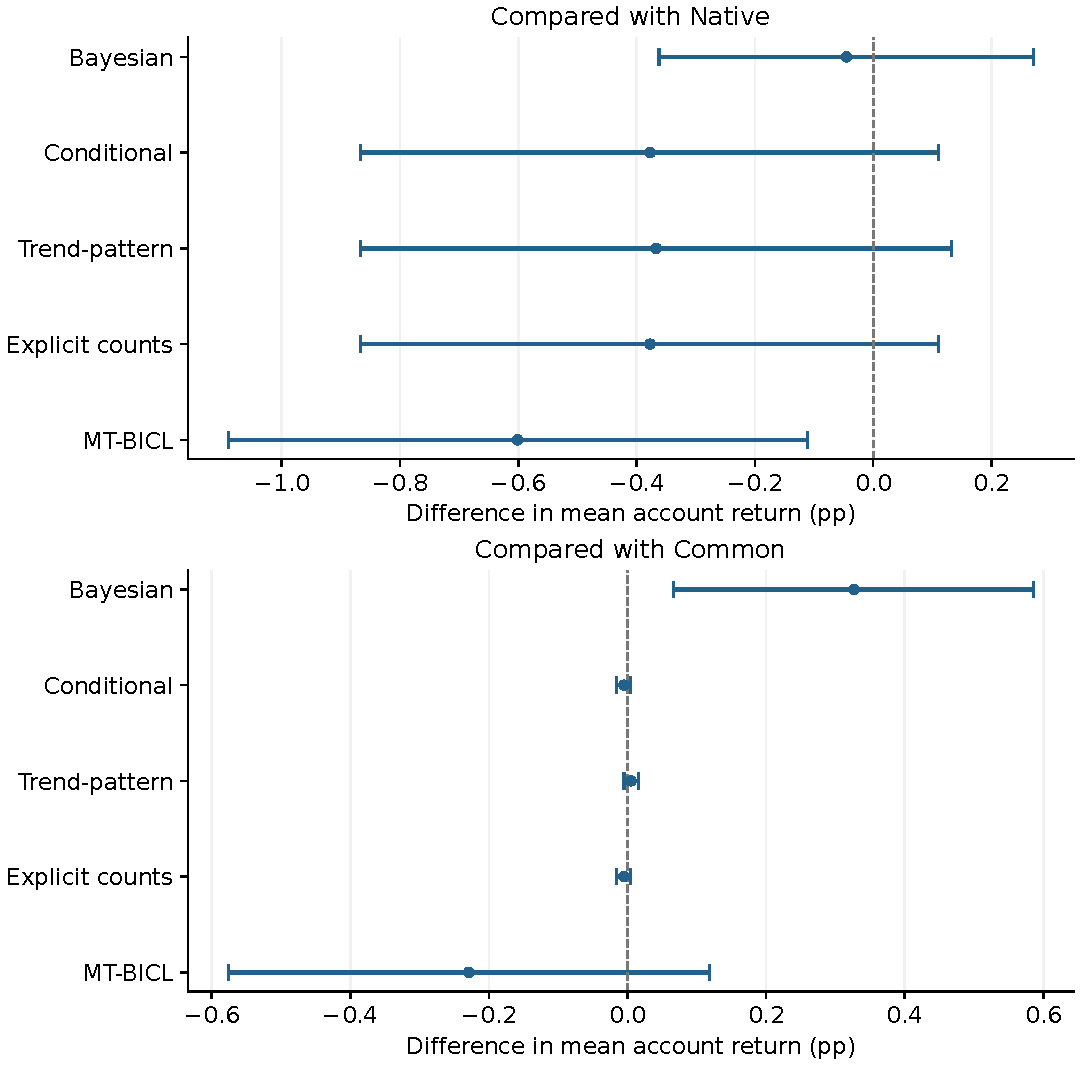
\includegraphics[width=0.84\textwidth,height=.40\textheight,keepaspectratio]{figures/return_comparisons.pdf}
\caption{Earlier historical-context study. Mean account-return differences against each augmented-system baseline, with descriptive simultaneous bands.}
\label{fig:u09-return-contrasts}
\end{figure}

BICL v2 and v4 each request only three new decisions across 306 slots.
Consequently, their aggregate outcomes mostly reflect fallback to Common.
BICL v5 agrees with Fact Anchor on 302 of 306 final actions. The three
successive comparisons in Table~\ref{tab:u09-bridge} show how much each
policy change affected actions and outcomes.

\paragraph{Follow-up historical-context evaluation}
The follow-up uses the same 102 cutoffs, a common causal alpha projection
and a rebuilt OHLCV memory bank. No news meets the historical
availability criterion on those dates. Five holding periods cross a
corporate action and one required entry has zero matched volume. Table%
~\ref{tab:bicl-complete-accounts} therefore compares the 45 accounts per
repeat with two labeled cycles, covering 90 cutoffs per repeat.

% Chiếu từ kết quả đã khóa của lần đánh giá bổ sung.
\begin{table}[!htb]
\centering\small
\caption{Follow-up BICL comparison on accounts with both trading cycles.}\label{tab:bicl-complete-accounts}
\begin{tabular}{lrrr}\toprule
Method & Mean net return (\%) & Balanced accuracy (\%) & Fallbacks / 306 \\ \midrule
Our system & -0.9379 & 46.2121 & 0 \\
Our system (Common) & -0.5304 & 53.2828 & 0 \\
BICL v1 & -0.5315 & 52.3990 & 162 \\
BICL v2 & -0.5177 & 53.7879 & 300 \\
BICL v3 & -0.5304 & 53.2828 & 282 \\
BICL v4 & -0.5177 & 53.7879 & 300 \\
BICL v5 & -1.0600 & 44.3182 & 117 \\
Fact Anchor & -1.0257 & 45.0758 & 0 \\
\bottomrule\end{tabular}
\par\smallskip
{\footnotesize Each repeat includes 45 of 51 accounts with both cycles, covering 90 cutoffs shared by all methods. Across the full sample, 96 of 102 cutoffs have valid execution labels.\par}
\end{table}


Mean-return differences for BICL v1--v4 versus Common range from
$-0.0011$ to $+0.0127$ pp. BICL v5 returns $-1.0600$\%, or $-0.1221$
and $-0.5297$ pp relative to Our system and Common, respectively.
The comparison uses owner-attested prices. The timing of historical
availability still needs independent verification.

\subsection{Component Contrasts and Variability}
Table~\ref{tab:repeats} reports a panel that regenerates chart reports and
a separate panel that holds the reports fixed while changing the
evidence shown to Decision. Each uses nine observations and three
executions. With a fixed upstream, the two-report branch trails
QuantAgent by 9.52 pp in balanced accuracy and the donor-value
variant by 11.90 pp. All seven descriptive factorial intervals include
zero. With regenerated reports, the paired difference is $+4.76$ pp
with a descriptive percentile interval of $[0,10]$ pp. The panels use
different cutoffs and cannot be combined to estimate variability for
the main 102-point cohort.

\begin{table}[!htb]
\centering\small
\renewcommand{\arraystretch}{1.13}
\caption{Component comparisons in two nine-observation panels. Cells are mean and sample SD across three executions.}
\label{tab:repeats}
\begin{tabular}{@{}llrr@{}}
\toprule
Panel & Method & BA (\%) & Net return (\%)\\
\midrule
Regenerated reports & QuantAgent & $90.48\pm 10.91$ & $0.37\pm 0.38$\\
 & Our system & $95.24\pm 4.12$ & $0.50\pm 0.22$\\
\addlinespace
Fixed reports & QuantAgent & $28.57\pm 7.14$ & $-1.70\pm 0.55$\\
 & Alpha only & $19.05\pm 4.12$ & $-2.03\pm 0.31$\\
 & Sentiment only & $14.29\pm 0.00$ & $-2.34\pm 0.22$\\
 & Our system & $19.05\pm 10.91$ & $-2.23\pm 0.63$\\
 & Past-donor alpha and sentiment & $30.95\pm 4.12$ & $-1.42\pm 0.33$\\
\bottomrule
\end{tabular}
\end{table}


\subsection{Robustness and Sensitivity}
Balanced accuracy varies across stocks and cutoffs
(Table~\ref{tab:symbol_results}). VNM has only DOWN observations, so
stock-level balanced accuracy is omitted there. On the common eight
stocks, the Our system--QuantAgent BA difference is $+2.08$ pp on 96
observations. Restricting the comparison to the three recent blocks
gives $+6.41$ pp on 54 observations. These overlapping cohorts share
dates and shocks.

Execution assumptions can change the return ordering. Higher costs
reverse the ordering under the reference ledger (Table~\ref{tab:execution}).
The additional comparisons in \ref{app:additional} use the same paired
forecasts. Repeated Decision calls and resampling quantify variability
conditional on the recorded dates and upstream realization.
